\documentclass[11pt,a4paper]{article}

\usepackage[T1]{fontenc}
\usepackage[czech]{babel}

\usepackage{amsmath}
\usepackage{amsfonts}
\usepackage{amssymb}
\usepackage{graphicx}
\usepackage[left=2cm,right=2cm,top=2cm,bottom=3.5cm]{geometry}
\usepackage{hyperref}
\usepackage{url}
\usepackage{url}
\usepackage[]{algorithm2e}
\usepackage[toc,page]{appendix}

% Colors
% ********************************************************************
\PassOptionsToPackage{dvipsnames}{xcolor}
\RequirePackage{xcolor} % [dvipsnames] 
\definecolor{halfgray}{gray}{0.55} % chapter numbers will be semi transparent .5 .55 .6 .0
\definecolor{webgreen}{rgb}{0,.5,0}
\definecolor{webbrown}{rgb}{.6,0,0}
\definecolor{Maroon}{cmyk}{0, 0.87, 0.68, 0.32}
\definecolor{RoyalBlue}{cmyk}{1, 0.50, 0, 0}
\definecolor{Black}{cmyk}{0, 0, 0, 0}


\hypersetup
{
bookmarksopen=true,
pdftitle="libGeoReport",
pdfauthor="Michal ELIAS",
pdfsubject="coordinate transformations",
pdftoolbar=true, % toolbar hidden
pdfmenubar=true, %menubar shown
pdfhighlight=/O, %effect of clicking on a link
colorlinks=true, %couleurs sur les liens hypertextes
pdfpagemode=None, %aucun mode de page
pdfpagelayout=SinglePage, %ouverture en simple page
pdffitwindow=true, %pages ouvertes entierement dans toute la fenetre
linkcolor=linkcol, %couleur des liens hypertextes internes
citecolor=citecol, %couleur des liens pour les citations
%urlcolor=linkcol %couleur des liens pour les url
colorlinks=true, breaklinks=true, bookmarks=true,bookmarksnumbered,
urlcolor=webbrown, linkcolor=RoyalBlue, citecolor=webgreen, % Link colors
}

\usepackage{fancyhdr} 
\pagestyle{fancy}
\fancyhf{}
\renewcommand{\headrulewidth}{0pt} % customise the layout...
\chead{ERA PROPRIETARY – NOT FOR DISTRIBUTION}\lhead{}\rhead{}
\cfoot{ERA PROPRIETARY – NOT FOR DISTRIBUTION}\lfoot{}\rfoot{}

\renewcommand{\contentsname}{Obsah}

\title{\normalfont{libGeo: Popis souřadnicových systémů a transformace mezi vybranými systémy}}
\author{\textsc{Michal Eliaš}}
\date{}

\begin{document}

\maketitle

\setcounter{tocdepth}{2} 


% Tabulka zmien dokumentu
\begin{table}[ht!]
\centering
\begin{tabular}{c|c|c|c}
\hline
Verze & Dátum & Autor & Opis změn \\
\hline
\hline
[0.1] & 2021-04-29 & mel & Práce na popisu transformace ECEF2ENU a ENU2ECEF\\
\hline
[0.2] & 2021-04-30 & mel & Dokončení ECEF2ENU a ENU2ECEF; doplnění příkladů \\
\hline
[0.3] & 2021-05-03 & mel & Popis trans. kov. matíc; Popis souř. systémů; doplnění pseudokódů \\
\hline

\end{tabular}
\end{table}

\tableofcontents % Print the table of contents

\listoffigures % Print the list of figures

\listoftables % Print the list of tables

\section*{Abstrakt}
\textit{
Dokument obsahuje popis transformací mezi vybranými souřadnicovýmí systémy.
}

\newpage 


\section*{Přehled důležitějších zkratek}

\begin{table}[ht!]
  \begin{tabular}{c c l}
    CTP  & - & Conventional Terrestrial Pole  \\
    ECEF & - & Earth-Centered Earth-Fixed. Pravouhlý souřadnicový systém \\
  & - & \\   
    IERS & - & International Erath Rotation Service \\
  \end{tabular}
\end{table}

\section*{Přehled důležitějších symbolů}

\begin{table}[ht!]
  \begin{tabular}{c c l}
    TBA  & - & TBA  \\
  \end{tabular}
\end{table}

\section{Úvod}

Dokument obsahuje základní popis transformací mezi vybranými souřadný systémy. Konkrétně se jedná o tyto souřadné soustavy:

\begin{enumerate}
\item ECEF (Earth Centred Earth Fixed) je pravoúhlá geocentrická souřadnicová soustava.
\item ENU (East North Up) je pravoúhlá lokální souřadnicová soustava.
\item GEOD je soustava geodetických/elipsoidickou souřadnic definovaných na rotačním elipsoidu, např. WGS-84.
\item SPHERE je soustava sférických souřadníc
\end{enumerate}

\subsection{Rešerš literatúry}

\subsubsection{Obecná četba}

TBA

\subsubsection{Zajímavé odkazy na literatúru ve vztahu k transformacím}

TBA 

\section{Poznámky}

\subsection{Transformace}

Definujme si zápis transformační matice ze souřadného systému UVW do souřadného systému XYZ například ve tvaru $\mathbf{C}_{XYZ}^{UVW}$ \cite{Grewal2001}.

Dále, ať vektor $\mathbf{v}$ obsahuje souřadnice systému XYZ, t.j. $\mathbf{v} = \left[v_{x}, v_{y}, v_{z}\right]^{T}$ a ten stejný vektor $\mathbf{v}$ ať obsahuje souřadnice $\mathbf{v} = \left[v_{u}, v_{v}, v_{w}\right]^{T}$ systému UVW. Pak pre obecný zápis transformace platí tento předpis

\begin{equation}
\begin{bmatrix}
v_{x} \\
v_{y} \\
v_{z}
\end{bmatrix} = \mathbf{C}^{UVW}_{XYZ}
\begin{bmatrix}
v_{u} \\
v_{v} \\
v_{w}
\end{bmatrix}
\label{rov:transGeneral}
\end{equation}
Systémy \textit{XYZ}, respektive \textit{UVW} reprezentují trojdimenzionální kartézské souřadné systémy.

Komponenty vektorů v jakémkoli souřadnícovém systému lze vyjádřit pomocí jejich jednotkových vektorů rovnoběžných s jejich příslušnými souřadnicovými osami. Například, ať souřadnicové osy systému XYZ označíme X, Y a Z a souřadnicové osy systému UVW označíme U, V a W, potom vektor \textbf{v} můžeme vyjádřit ve tvaru

\begin{eqnarray}
\mathbf{v} &=& v_{x}\mathbf{1}_{x} + v_{y}\mathbf{1}_{y} + v_{z}\mathbf{1}_{z} \\ \nonumber
           &=& v_{u}\mathbf{1}_{u} + v_{v}\mathbf{1}_{v} + v_{w}\mathbf{1}_{w}, 
\end{eqnarray}
kde
\begin{itemize}
\item jednotkové vektory $\mathbf{1}_{x}, \mathbf{1}_{y}, \mathbf{1}_{z}$ jsou definovány podél souřadných os X, Y a Z systému XYZ,
\item skaláry $v_{x}, v_{y}, v_{z}$ jsou komponenty vektoru \textbf{v} definovány podél souřadných os X, Y a Z systému XYZ,
\item jednotkové vektory $\mathbf{1}_{u}, \mathbf{1}_{v}, \mathbf{1}_{w}$ jsou definovány podél souřadných os U, V a W systému UVW, 
\item skaláry $v_{u}, v_{v}, v_{w}$ jsou komponenty vektoru \textbf{v} definovány podél souřadných os U, V a W systému UVW. 
\end{itemize}

Příslušné komponenty vektoru lze vyjádřit pomocí skalárního součinu příslušných jednotkových vektorů, například ve tvaru

\begin{eqnarray}
v_{x} &=& \mathbf{1}^{T}_{x}\mathbf{v} = v_{u}\mathbf{1}^{T}_{x}\mathbf{1}_{u} + v_{v}\mathbf{1}^{T}_{x}\mathbf{1}_{v} + v_{w}\mathbf{1}^{T}_{x}\mathbf{1}_{w}, \\
v_{y} &=& \mathbf{1}^{T}_{y}\mathbf{v} = v_{u}\mathbf{1}^{T}_{y}\mathbf{1}_{u} + v_{v}\mathbf{1}^{T}_{y}\mathbf{1}_{v} + v_{w}\mathbf{1}^{T}_{y}\mathbf{1}_{w}, \\
v_{z} &=& \mathbf{1}^{T}_{z}\mathbf{v} = v_{u}\mathbf{1}^{T}_{z}\mathbf{1}_{u} + v_{v}\mathbf{1}^{T}_{z}\mathbf{1}_{v} + v_{w}\mathbf{1}^{T}_{z}\mathbf{1}_{w},
\end{eqnarray}
a v maticové formě předchozí rovnice nabývají tento zápis

\begin{equation}
\begin{bmatrix}
v_{x} \\
v_{y} \\
v_{z}
\end{bmatrix} =
\begin{bmatrix}
\mathbf{1}_{x}^{T}\mathbf{1}_{u} & \mathbf{1}_{x}^{T}\mathbf{1}_{v} & \mathbf{1}_{x}^{T}\mathbf{1}_{w} \\
\mathbf{1}_{y}^{T}\mathbf{1}_{u} & \mathbf{1}_{y}^{T}\mathbf{1}_{v} & \mathbf{1}_{y}^{T}\mathbf{1}_{w} \\
\mathbf{1}_{z}^{T}\mathbf{1}_{u} & \mathbf{1}_{z}^{T}\mathbf{1}_{v} & \mathbf{1}_{z}^{T}\mathbf{1}_{w} 
\end{bmatrix} 
\begin{bmatrix}
v_{u} \\
v_{v} \\
v_{w}
\end{bmatrix} = \mathbf{C}^{UVW}_{XYZ}
\begin{bmatrix}
v_{u} \\
v_{v} \\
v_{w}
\end{bmatrix}.
\label{rov:transGeneral}
\end{equation}

Tímto jsme si odvodili souřadnicovou transformační matici $\mathbf{C}_{XYZ}^{UVW}$. Skalární součin jednotkových ortogonálních vektorů umožňuje odvodit směrové kosiny, přičemž obecně platí, že

\begin{equation}
\mathbf{1}^{T}_{a}\mathbf{1}_{b} = \cos{\left(\theta_{a, b}\right)}.
\end{equation}
V důsledku toho, souřadnicová transformační matice může být vyjádřena ve tvaru
\begin{equation}
\mathbf{C}_{XYZ}^{UVW} = 
\begin{bmatrix}
\cos{\left(\theta_{x,u}\right)} \cos{\left(\theta_{x,v}\right)} \cos{\left(\theta_{x,w}\right)} \\
\cos{\left(\theta_{y,u}\right)} \cos{\left(\theta_{y,v}\right)} \cos{\left(\theta_{y,w}\right)} \\
\cos{\left(\theta_{z,u}\right)} \cos{\left(\theta_{z,v}\right)} \cos{\left(\theta_{z,w}\right)} 
\end{bmatrix}.
\label{rov:generRotMat}
\end{equation}
Rovnice \ref{rov:generRotMat} vyjadřuje všeobecnou rotační matici v trojrozměrném prostoru.

\subsection{Translace}

V předchozí kapitole jsme se věnovali podobnostnej transformaci mezi dvěma pravoúhlými souřadný systémy. V případě posunu (translace), počátek jedné soustavy do počátku druhé soustavy jednoznačně vyjádříme pomocí vektoru

\begin{equation}
\mathbf{r} = 
\begin{bmatrix}
\left(x-u\right) & \left(y-v\right) & \left(z-w\right)
\end{bmatrix}^{T}.
\end{equation}

\subsection{Transformace kovariančních matíc}

Cílem kapitoly je navrhnout transformaci kovariančních matic souřadnic (jejích přesností) mezi uvažovanými souřadnými systémy. Princip postupu je založen na zákoně hromadění středních chyb, viz například \cite{Kubacek2013} anebo \cite{Mikhail1976}.

Matematický zápis transformace kovarianční matice mezi vybranými systémy je tento:

\begin{equation}
\mathbf {\Sigma}_{XYZ} = \mathbf{J} \mathbf{\Sigma}_{UVW} \mathbf{J}^{T},
\end{equation}
kde
\begin{itemize}
\item $\mathbf{J}$ je Jakobi matice příslušné transformace,
\item $\mathbf{\Sigma}_{UVW}$ je kovarianční matice souřadnic resp. souřadného systému, ze kterého transformujeme a
\item $\mathbf{\Sigma}_{XYZ}$ je kovarianční matice souřadnic resp. souřadného systému, do kterého transformujeme.
\end{itemize}

\newpage
\subsection{Súradnicové systémy}


\subsubsection{ECEF - Earth Centred Earth Fixed}

\begin{figure}[ht!]
\begin{center}

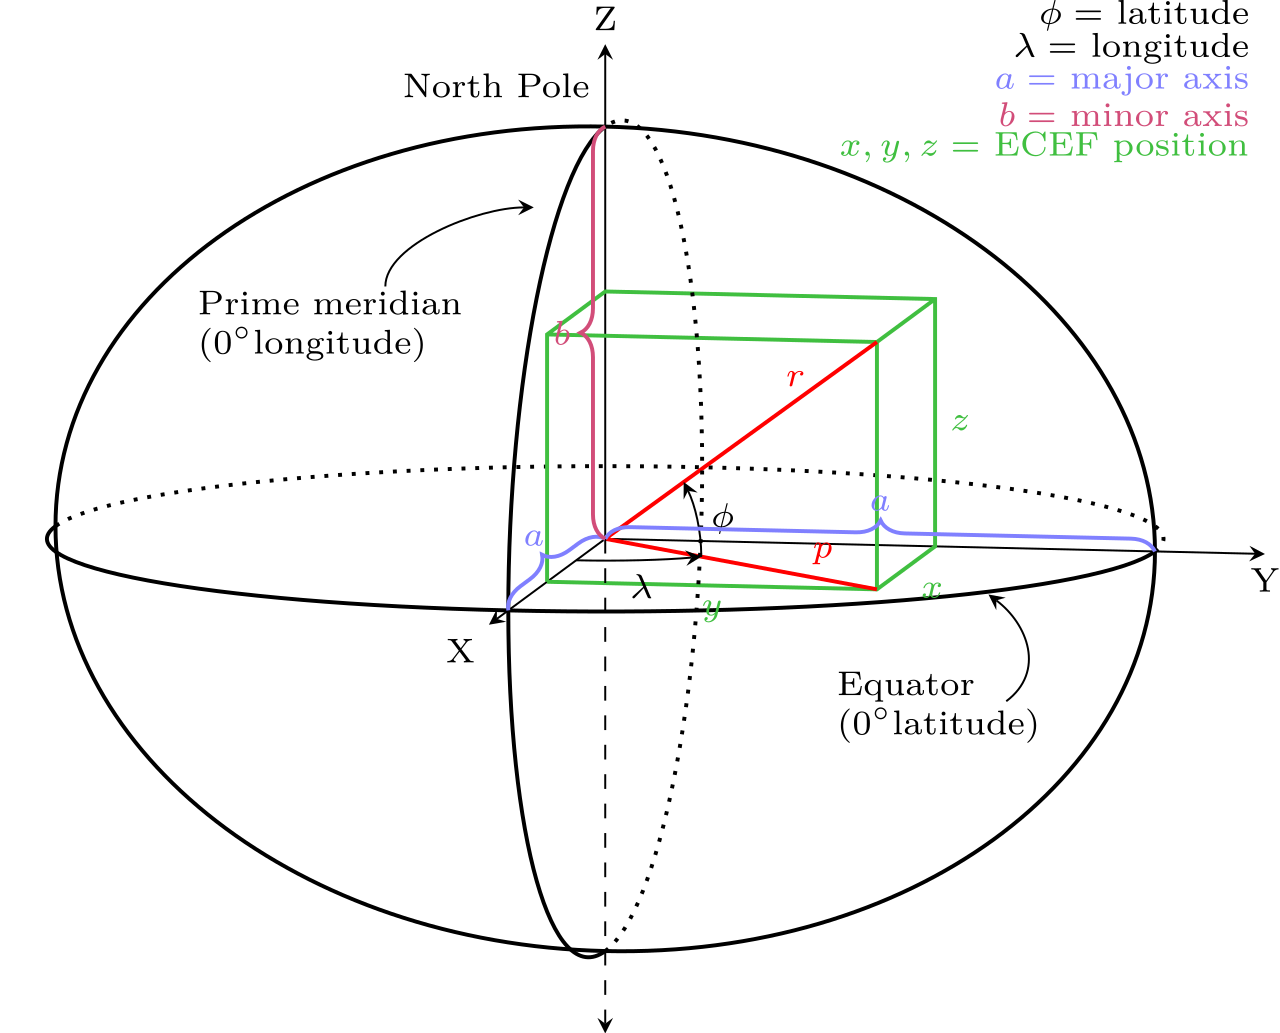
\includegraphics[width=0.60\textwidth]{FIG/ecef_wiki}
\caption{Zobrazení bodu v ECEF soustavě souřadnic. Obrázek je převzat z \cite{ecefWiki}.}
\label{fig:ecef}
\end{center}
\end{figure}

Základní kartézská pravouhlá soustava souřadníc, naúříklad tak, jako je zobrazená na obrázku \ref{fig:ecef}, je definována takto \cite{Soler1988}, \cite{Kovar2016}:

\begin{itemize}
\item počátek soustavy je soustředěn v geocentre, t.j. v gravitačním středu zemského tělesa,
\item osa \textbf{Z} směruje do místa zemského severního pólu, který je definován podle IERS. Protože poloha pólu sa v čase mění, používá se střední poloha zemského pólu (CTP).
\item osa \textbf{X} prochází bodem nulové zeměpisné délky, t.j. Greenwich poledníkem, který je definován podle IERS a míři do průsečníku tohto poledníku a roviny rovníku,
\item osa \textbf{Y} doplňuje pravotočivý pravouhlý sýstém souřadníc.
\end{itemize}

\subsubsection{ENU - East-North-Up}

Některé výpočty souřadníc je praktičtější provádět v lokální souřadnicové soustavě například vzdálenosť radarového přijímače od daného bodu atp.,\cite{Kovar2016}, \cite{Mayer2002}. ENU je lokální pravouhlá soustava souřadnic, pričemž její definice a umístnění počátku soustavy a souřadnicových os, dle značení na obrázku \ref{fig:enu}, jsou:
 
\begin{itemize}
\item počátek systému soustavy souřadníc je umiestnený v středě regiónu záujmu a to  buď na povrchu anebo blízko povrchu referenčního tělesa (elipsoid, koule),
\item osa \textbf{n} (North) směruje na sever, 
\item osa \textbf{e} (East) směruje na východ a 
\item osa \textbf{u} (Up) je totožná s normálou referenčního tělesa (elipsoid, koule). 
\end{itemize}

\begin{figure}[ht!]
\begin{center}

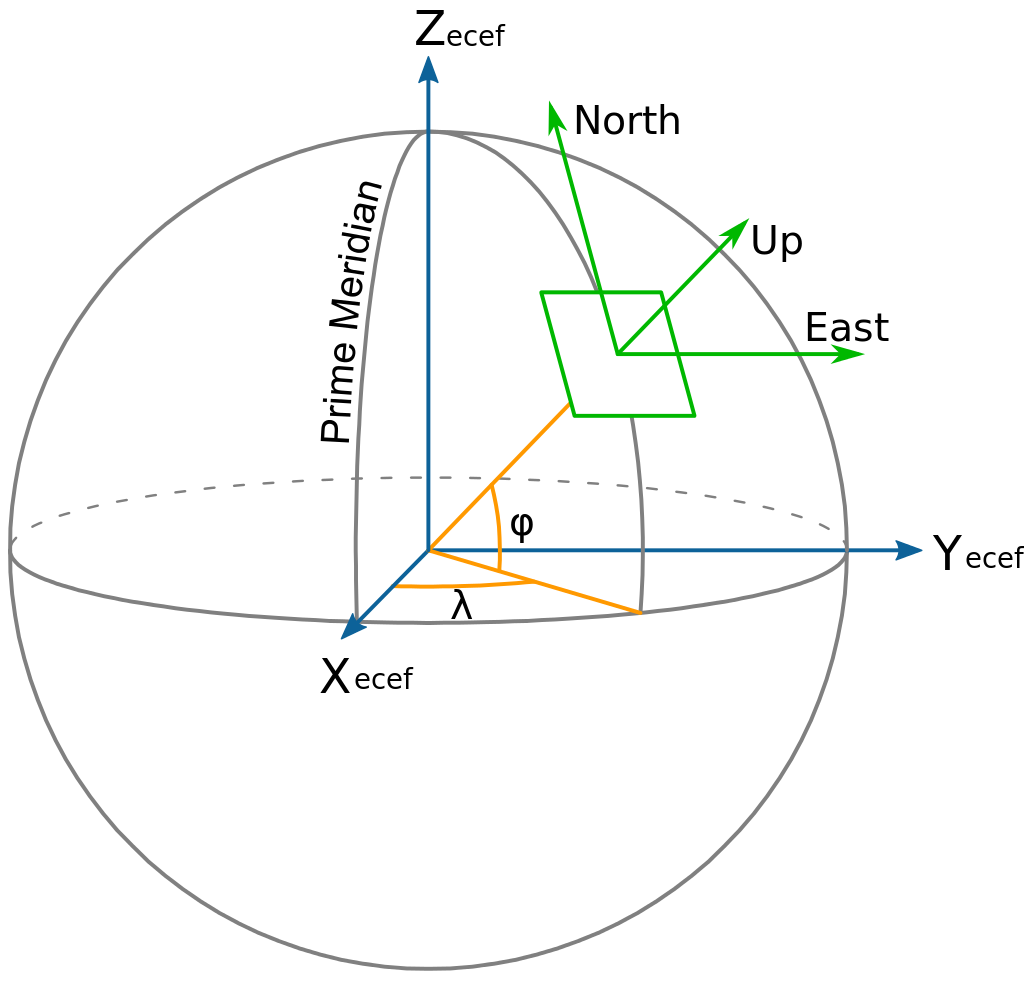
\includegraphics[width=0.50\textwidth]{FIG/enu_wiki}
\caption{Zobrazení systému souřadnic East-North-Up. Obrázek je převzat z \cite{enuWiki}.}
\label{fig:enu}
\end{center}
\end{figure}

\subsubsection{GEOD - Systém geodetických souřadníc}

\begin{figure}[ht!]
\begin{center}
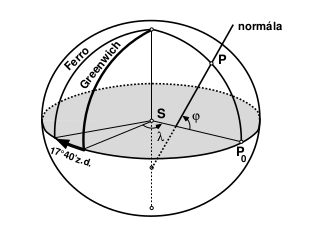
\includegraphics[width=0.50\textwidth]{FIG/geod_cimb}
\caption{Geodetické zeměpisné souřadnice. Obrázek je převzat z \cite{Cimbalnik1997}.}
\label{fig:geod}
\end{center}
\end{figure}

V praktických úlohách se poloha bodu popisuje pomocí geodetických anebo elipsoidických souřadníc. Elipsoidických proto, protože se definuje pomocí zvoleného zemského elipsoidu. Ten slouží k aproximaci fyzického zemského tělesa. Základní matematické vzorce určené pro odvození elipsoidu jsou obsahem přílohy \ref{appRefEll} a přehled konstant globálne užitých elipsoidů jsou obsahem přílohy \ref{appRefEllConst}.

Poloha bodu \textbf{P} na obrázku \ref{fig:geod} se vyjadřuje třemi souřadnicemi:

\begin{enumerate}
\item geodetickou zeměpisnou šířkou $\varphi$,
\item geodetickou zeměpisnou délkou $\lambda$,
\item geodetickou výškou.
\end{enumerate} 

Geodetická zeměpisná šířka $\varphi$ bodu \textbf{P} je uhel, který svírá normála v bodě P k povrchu elipsoidu, s rovinou rovníku. Geodetická zeměpisná délka $\lambda$ je úhel, který svírá rovina poledníku tohoto bodu s rovinou nultého poledníku. Za nultý poledník je mezinárodně volen ten, který prochází stabilizovaným bodem na astronomické observatoři v Greenwich. Geodetická výška se měří podél normály mezi referenčním elipsoidem a bodem \textbf{P}.

\subsubsection{SPHERE - Systém sférických (polárnych) súradníc}

Koule je základní a nejjednoduchší aproximace zemského tělesa. Sférické souřadnice tvoří systém souřdnic, které popisujou polohu bodu na sféře. Referenční koule je pak definovaná sférickým poloměrem. Pro praktické výpočty se jeho hodnota často zpočíta jako středný pomoměr křivosti (a to z důvodu zachování objemu eliposidu během jeho zobrazení na kouli, t.j. v místě lokálni aproximace - viz příloha \ref{appRefEll}).
 
\begin{figure}[ht!]
\begin{center}
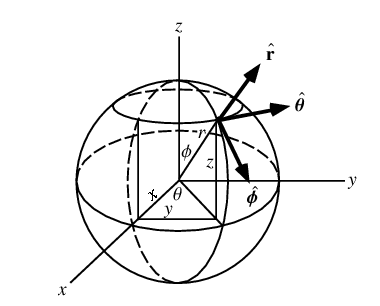
\includegraphics[width=0.50\textwidth]{FIG/sphere_wolf}
\caption{Sférické polárni souřadnice. Obrázek je převzat z \cite{sphereWolf}.}
\label{fig:sphere}
\end{center}
\end{figure}

Dle situace zobrazené na obrázku \ref{fig:sphere}, poloha bodu na sféře je vyjadřená soustavou tří souřadníc:
\begin{itemize}
\item $\theta$ hodnota azimutu v rovině rovníka. Pokud je uhel značený symbolem $\lambda$, pak poukazuje na zeměpisnou délku,
\item $\phi$ hodnota polárniho úhla počítaná od zenitu (také zenitový úhel). Pokud je uhel značený symbolem $\varphi^{'}$, pak poukazuje na doplnek zemepisej délky od zenitu, t.j. $\varphi = 90 - \varphi^{'}$ a
\item r, je středný polomer Zeme.
\end{itemize}

\section{Transformace souřadníc medzi vybranými souřadnicovými soustavami}

\subsection{ECEF $\rightarrow$ ENU $\&$ ENU $\rightarrow$ ECEF}

Předpokládejme, že v tomto příkladu je uvažovaný rotační elipsoid (například WGS-84 nebo GRS-80) geocentrický, to znamená, že střed elipsoidu se nachází ve středu zemského tělesa. Transformace souřadnic pak mezi zemským geocentrickým systémem souřadnic (xyz) a lokálním topocentrickým (nebo také lokálním geodetickým - enu) systémem může být vyjádřený předpisem \cite{Soler1998}

\begin{equation}
\begin{bmatrix}
e \\
n \\
u
\end{bmatrix} = 
\mathbf{C}_{enu}^{xyz}
\begin{bmatrix}
x \\
y \\
z
\end{bmatrix}.
\label{rov:ecef2enu1}
\end{equation}

Pro popis transformace mezi uvedenými systémy si potřebujeme odvodit transformační matici, v tomto případě takzvanou rotační matici. Vycházejme z rovnice \ref{rov:generRotMat}. Rotační matici pak zostavíme pro rotaci v prostoru a to pomocí jednoduchých rotací v každé ose samostatně.

Rotační matice kolem osy \textit{z} ve směru hodinových ručiček nabude tvar
\begin{equation}
\mathbf{R_{3}}\left(\theta\right) = 
\begin{bmatrix}
\cos{\left(\theta\right)} & \sin{\left(\theta\right)} & 0 \\
-\sin{\left(\theta\right)} & \cos{\left(\theta\right)} & 0 \\
0 & 0 & 1
\end{bmatrix},
\end{equation}
přičemž rotace kolem osy \textit{z} je $\cos{\left(\theta_{z, w} \right)} = \cos{\left(0\right)} = 1$, protože úhel mezi osama \textit{z} a \textit{w}, které jsou v tomto přikladě totožné, je roven nule. Dále platí, že kosinus úhlu $ \cos{\left(\theta_{z, u} \right)}= \cos{\left(90\right)} = 0 $, protože \textit {z} a \textit {u} jsou na sebe kolmé. Stejně tento předpoklad platí i pro $\cos{\left(\theta_{z,v}\right)}$, $\cos{\left(\theta_{x,w}\right)}$ a $\cos{\left(\theta_{y,w}\right)}$.

Analogicky postup bude platit i pro ostatní dvě rotace a tedy rotace kolem osy \textit{x} je
\begin{equation}
\mathbf{R_{1}}\left(\theta\right) = 
\begin{bmatrix}
1 & 0 & 0 \\
0 &  \cos{\left(\theta\right)} & \sin{\left(\theta\right)} \\
0 & -\sin{\left(\theta\right)} & \cos{\left(\theta\right)} \\
\end{bmatrix},
\end{equation}
a kolem osy \textit{y}
\begin{equation}
\mathbf{R_{2}}\left(\theta\right) = 
\begin{bmatrix}
\cos{\left(\theta\right)} & 0 & -\sin{\left(\theta\right)} \\
0 & 1 & 0 \\
\sin{\left(\theta\right)} & 0 & \cos{\left(\theta\right)} \\
\end{bmatrix},
\end{equation}

Vyjádření transformační matice $\mathbf {C}_{enu}^{xyz} $ mezi dvěma pravoúhlými kartézskymi souřadnicovými systémy ECEF a ENU je založen na součinu dvou rotací, konkrétně:
\begin{enumerate}
\item rotaci kolem osy \textit{z} o úhel $\pi/2 + \lambda $ a
\item rotaci kolem osy \textit{y} o úhel $\pi/2 - \varphi $,
\end{enumerate}
kde úhlové stupně $\lambda$, respektíve $\varphi$ geograficky představují stupeň otočení jedné soustavy od druhé ve směru zeměpisné délky ($\lambda$) a ve směru zeměpisné šířky ($\varphi$).

Potom transformace mezi systémy se dá vyjádřit ve tvaru

\begin{equation}
\begin{bmatrix}
e \\
n \\
u
\end{bmatrix} =
\mathbf{R_{1}}\left(\pi/2-\varphi\right)\mathbf{R_{3}}\left(\pi/2+\lambda\right)
\begin{bmatrix}
x \\
y \\
z
\end{bmatrix} =
\begin{bmatrix}
-\sin{\left(\lambda\right)} & \cos{\left(\lambda\right)} & 0 \\
-\cos{\left(\lambda\right)}\sin{\left(\varphi\right)} & -\sin{\left(\lambda\right)}\sin{\left(\varphi\right)} & \cos{\left(\varphi\right)} \\
\cos{\left(\lambda\right)}\cos{\left(\varphi\right)} & \sin{\left(\lambda\right)}\cos{\left(\varphi\right)} & \sin{\left(\varphi\right)}
\end{bmatrix}
\begin{bmatrix}
x \\
y \\
z
\end{bmatrix}.
\label{rov:ecef2enu2}
\end{equation}

Jednou z vlastností rotačných matíc je tá, podle které $\mathbf{R}\left(\theta\right)^{-1} = \mathbf{R}\left(-\theta\right) = \mathbf{R}\left(\theta\right)^{T}$. Z toho plyne, že zápis pro inversnou tranformaci je

\begin{equation}
\begin{bmatrix}
x \\
y \\
z
\end{bmatrix} =
\mathbf{R_{3}}\left(-\left(\pi/2+\lambda\right)\right)\mathbf{R_{1}}\left(-\left(\pi/2-\varphi\right)\right)
\begin{bmatrix}
e \\
n \\
u
\end{bmatrix} = 
\begin{bmatrix}
-\sin{\left(\lambda\right)} & -\cos{\left(\lambda\right)}\sin{\left(\varphi\right)} & \cos{\left(\lambda\right)}\cos{\left(\varphi\right)} \\
 \cos{\left(\lambda\right)} & -\sin{\left(\lambda\right)}\sin{\left(\varphi\right)} & \sin{\left(\lambda\right)}\cos{\left(\varphi\right)} \\
 0  &  \cos{\left(\varphi\right)} & \sin{\left(\varphi\right)} 
\end{bmatrix}
\begin{bmatrix}
e \\
n \\
u
\end{bmatrix}.
\label{rov:ecef2enu3}
\end{equation}

Z předchozího zápisu plyne, že během rotace pravoúhlých souřadnicových soustav předpokládáme, že počátky souřadnic jsou shodné. V případě, že počátek, například soustavy ENU umístíme na povrch referenčního tělesa (elipsoid případně sféry), je zapotřebí doplnit posun mezi soustavami. Potom rovnice \ref{rov:ecef2enu2} nabude tvar

\begin{equation}
\begin{bmatrix}
e \\
n \\
u
\end{bmatrix} =
\mathbf{R}
\begin{bmatrix}
x - x_{0} \\
y - y_{0} \\
z - z_{0}
\end{bmatrix},
\label{rov:ecef2enu22}
\end{equation}
a rovnici \ref{rov:ecef2enu3} doplníme do tvaru
\begin{equation}
\begin{bmatrix}
x \\
y \\
z
\end{bmatrix} =
\begin{bmatrix}
x_{0} \\
y_{0} \\
z_{0}
\end{bmatrix} + 
\mathbf{R}^{T}
\begin{bmatrix}
e \\
n \\
u
\end{bmatrix},
\label{rov:ecef2enu33}
\end{equation}
kde pravoúhlé souřadnice vektoru $\mathbf{r}_{0}=\left[x_{0}, y_{0}, z_{0} \right]$ získáme transformací zeměpisných souřadnic posunutého počátku například ENU soustavy ($\varphi$, $\lambda$, $hel$) do systému geocentrických kartézskych souřadnic (například systému ECEF).

\subsubsection{Příklad transformace z ECEF $\rightarrow$ ENU}

Nechť bod A je vyjádřen v souřadnicích souřadného systému ECEF a hodnoty souřadnic jsou:
\begin{itemize}
\item $x = 4198944.6161$ m
\item $y = 174747.2383$ m
\item $z = 4781886.8769$ m
\end{itemize}

Mějme bod B, jehož geodetické souřadnice jsou $ \varphi = 48.8862 deg$, $\lambda = 2.3343 deg$ a geodetická výška je $ h = 174.5217 m $. Úhlové souřadnice použijeme jednak k natočení souřadných soustav (viz rotační matice v rovnici \ref{rov:ecef2enu2}) a společně se zadanou elipsoidickou výškou, k umístění počátku ENU soustavy, který umístíme nad povrch rotačního elipsoidu. Úkolem je vyjádřit souřadnice bodu \textit{A} v soustavě ENU a s přihlédnutím definovaného počátku ENU soustavy v bodě B.

Vektor pravoúhlých souřadnic bodu B, tj $ \left(x_{0}, y_{0}, z_{0} \right)$ získáme transformací GEOD2ECEF(). ENU souřadnice bodu A s přihlédnutím k umístění počátku ENU soustavy v bodě B a vypočítané podle \ref{rov:ecef2enu22}, jsou:
\begin{itemize}
\item $e = 3579.4232 $ m
\item $n = -688.3514 $ m
\item $u = -51.0524 $ m.
\end{itemize}

Pseudokód Matlab funkce ecef2enu(), která je implementováná v package +Geo je stručně popsaná v příloze \ref{appEcef2Enu}.

\subsubsection{Příklad transformace z ENU $\rightarrow$ ECEF}

V tomto příkladě bude naší úlohou přezentovat inverzní transformaci, no vycházejme z výsledků výpočtu polohy bodu v ENU soustavě souřadnic, t.j. souřadníc pro bod B v předcházejícim příkladě. Jeho souřadnice jsou:

\begin{itemize}
\item $e = 3579.4232$ m
\item $n = -688.3514$ m
\item $u = -51.0524$ m.
\end{itemize}


Dle rovnice \ref{rov:ecef2enu33}, ECEF XYZ souřadnice bodu A jsou:
\begin{itemize}
\item $x = 4198944.6161$ m
\item $y = 174747.2383$ m
\item $z = 4781886.8769$ m.
\end{itemize}

Pseudokód Matlab funkce enu2ecef(), která je implmentováná v package +Geo Package je obsahem přílohy \ref{appEnu2Ecef}

\bibliographystyle{apalike}
\bibliography{zoznamLiteratury} 





\begin{appendices}

\section{Matematické vzorce odvozené na referenčním elipsoidu} \label{appRefEll}

TBA

\section{Konstanty základních referenčních elipsoidů} \label{appRefEllConst}

TBA

\section{Pseudokódy implementovaných transformácii v Matlab package +Geo}

\subsection{ECEF2ENU} \label{appEcef2Enu}

\begin{algorithm}[H]
 \KwData{x, y, z, $\varphi$, $\lambda$, hel, RT, ELL}
 \KwResult{e, n, u}
 výpočet rotační matice $\mathbf{R}\left(\varphi, \lambda\right)$\;	
 \eIf{RT == elipsoid}{
  $[x_{0}, y_{0}, z_{0}] = geod2ecef(\varphi, \lambda, hel, ELL)$\;
  }{
  $[x_{0}, y_{0}, z_{0}] = sphere2ecef(\varphi, \lambda, hel^{*})$\;
 }
 Výpočet podle rovnice \ref{rov:ecef2enu22}
 \caption{Transformácia ECEF2ENU}
\end{algorithm} 

\subsection{ENU2ECEF} \label{appEnu2Ecef}

\begin{algorithm}[H]
 \KwData{e, n, u, $\varphi$, $\lambda$, hel, RT, ELL}
 \KwResult{x, y, z}
 výpočet rotační matice $\mathbf{R}\left(\varphi, \lambda\right)$\;	
 \eIf{RT == elipsoid}{
  $[x_{0}, y_{0}, z_{0}] = geod2ecef(\varphi, \lambda, hel, ELL)$\;
  }{
  $[x_{0}, y_{0}, z_{0}] = sphere2ecef(\varphi, \lambda, hel^{*})$\;
 }
 Výpočet podle rovnice \ref{rov:ecef2enu33}
 \caption{Transformácia ENU2ECEF}
\end{algorithm} 



\end{appendices}


\end{document}
